\documentclass[letterpaper, 10 pt]{article}

% For handling graphics
\usepackage{graphicx}
% For colors
\usepackage{color}
% For hyperlink
\usepackage{url}
\PassOptionsToPackage{hyphens}{url}
\usepackage{hyperref}
\hypersetup{
    colorlinks,
    linktoc=all,
    citecolor=black,
    filecolor=black,
    linkcolor=black,
    urlcolor=blue
}
% For mathematics
\usepackage{mathtools}
\usepackage[margin=1.0in]{geometry}
\usepackage{listings}

% Remove section numbering
\setcounter{secnumdepth}{0}

% -------------------------------------------------------------------------------------
% TITLE PAGE
% -------------------------------------------------------------------------------------
\begin{document}
\begin{titlepage}
\center
% Headings
\textsc{\LARGE PVLabs}\\[1.5cm]

% Title
\rule{\linewidth}{0.5mm}\\[0.4cm]
{\huge \bfseries PhantomX Reactor Arm Notebook}\\[0.4cm]
\rule{\linewidth}{0.5mm}\\[1.5cm]
% Author
\textsc{\normalsize Rapierevite}\\[1.5cm]
% Image
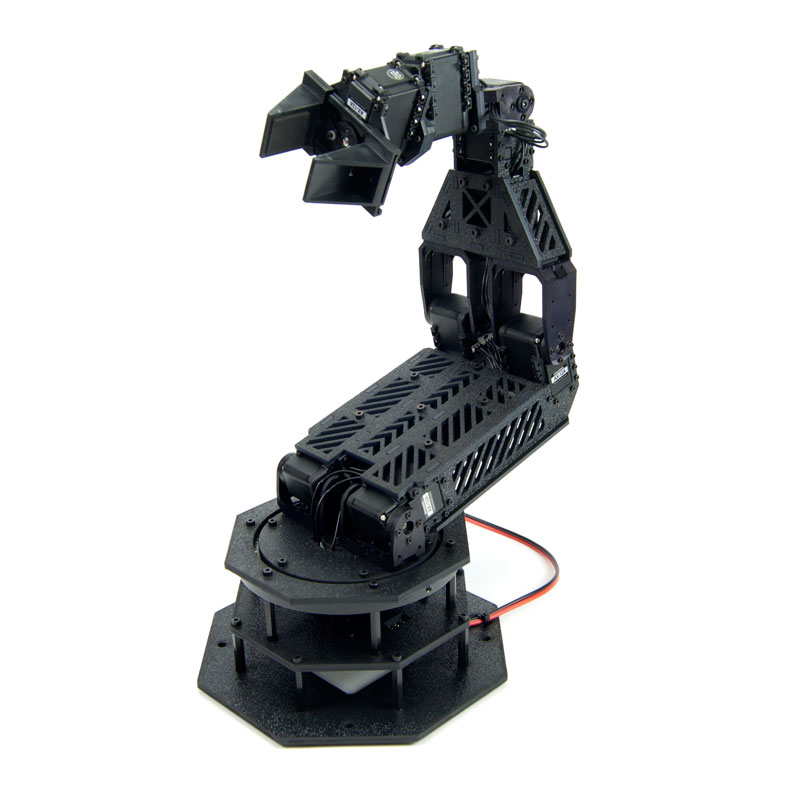
\includegraphics[width=10.0cm]{resources/phantomx-reactor}
% Fill rest of page with whitespace
\vfill
\end{titlepage}

\tableofcontents
\newpage


% -------------------------------------------------------------------------------------
% JOURNAL ENTRIES
% -------------------------------------------------------------------------------------

\section{Building the PhantomX Reactor Arm - 2014/05/11}
During the building of the PhantomX Reactor arm I came across and learned by mistake several things.
  \subsection{Dynamixel servo IDs}
    \begin{itemize}
    \item Set the ID of each servo individually using the dynamanager software before starting to build the robot arm. \url{http://learn.trossenrobotics.com/arbotix/arbotix-getting-started/1-setting-dynamixel-ids-with-the-dynamanager.html#&panel1-1}. I was not able to connect to the servos until I fixed an issue with the RXTXcomm.jar java file.
    \end{itemize}
  \subsection{Accessing the USB port on Linux, Ubuntu 12.04}
    \begin{itemize}
      \item The "Serial Port" menu inside the "Tools" menu in the Arduino IDE was greyed out. The problem occurs because of conflicting .jar files. Locate all "RXTXcomm.jar" files and figure out which one is the problem and remove it. For me it was a MATLAB version of the file.
      \item sudo updatedb (update the database)
      \item locate RXTXcomm.jar (locate the file) \newline
      /usr/share/arduino/lib/RXTXcomm.jar \newline
      /usr/share/java/RXTXcomm.jar
      \item I renamed the first one and restarted and everything work fine. I was able to see \textbf{/dev/ttyUSB0}
    \end{itemize}
  \subsection{Connection error}
    \begin{itemize}
      \item Before my computer could actually connect to the Arbotix I got the following error when I tried to upload test code: \textbf{"avrdude : stk500\_getsync():not in sync: resp=0x00"} \newline
      This error means the computer can't connect to the board. The fix was to hit the "reset" button on the Arbotix board and power cycle. After that I was able to upload just fine.
    \end{itemize}
  \subsection{Parts Screw-ups}
    \begin{itemize}
      \item One standoff was broken
      \item One screw head was melted and unusable
      \item The M2-14 screws were not grade 8 like all the other ones.
    \end{itemize}
  \subsection{Running Arduino Test Code from Sketchbook}
    \begin{itemize}
      \item The demo ran fine except that at the beginning the base servo shot to the middle position super fast and terrifyingly. And everytime I powered the arm on, it ran that same test program, so make sure it's in a safe location. The middle position of the servo (the ideal zero position) is located in between 0 and the limit (usually around 300 degrees).
    \end{itemize}

%------------------------

\section{Communicating With The Arm - 2014/05/12}
  \subsection{XBee Wifi Module}
    \begin{itemize}
      \item Buy the Wifi Trace or PCB version. \url{https://www.sparkfun.com/products/11215}. \$22.95.
      \item Requires USB-to-XBee adapter to program or communicate from a computer
      \item One XBee goes directly on the ArbotiX board and the other goes on the adapter that's plugged into the computer.
    \end{itemize}
  \subsection{USB2Dynamixel PC-to-Motors Adapter}
    \begin{itemize}
      \item \url{http://www.trossenrobotics.com/robotis-bioloid-usb2dynamixel.aspx} \$49.99.
      \item Provides communication between computer and Dynamixel motors. So the most logical setup would be to buy a BeagleBone Black and put it on the arm base and communicate with it using a client computer. The USB2Dynamixel adapter to connect to the BeagleBone Black or PandaBoard.
      \item Power is not supplied via USB so the best solution is to use the SMPS2Dynamixel power adapter.
    \end{itemize}
  \subsection{SMPS2Dynamixel Power Adapter}
    \begin{itemize}
      \item It is designed to provide power from the SMPS power supply but can also be powered by external power, such as a lithium ion battery.
    \end{itemize}
    
%------------------------

\section{Using ROS with Dynamixel - 2014/05/23}
  \subsection{Setup}
    \begin{center}
  	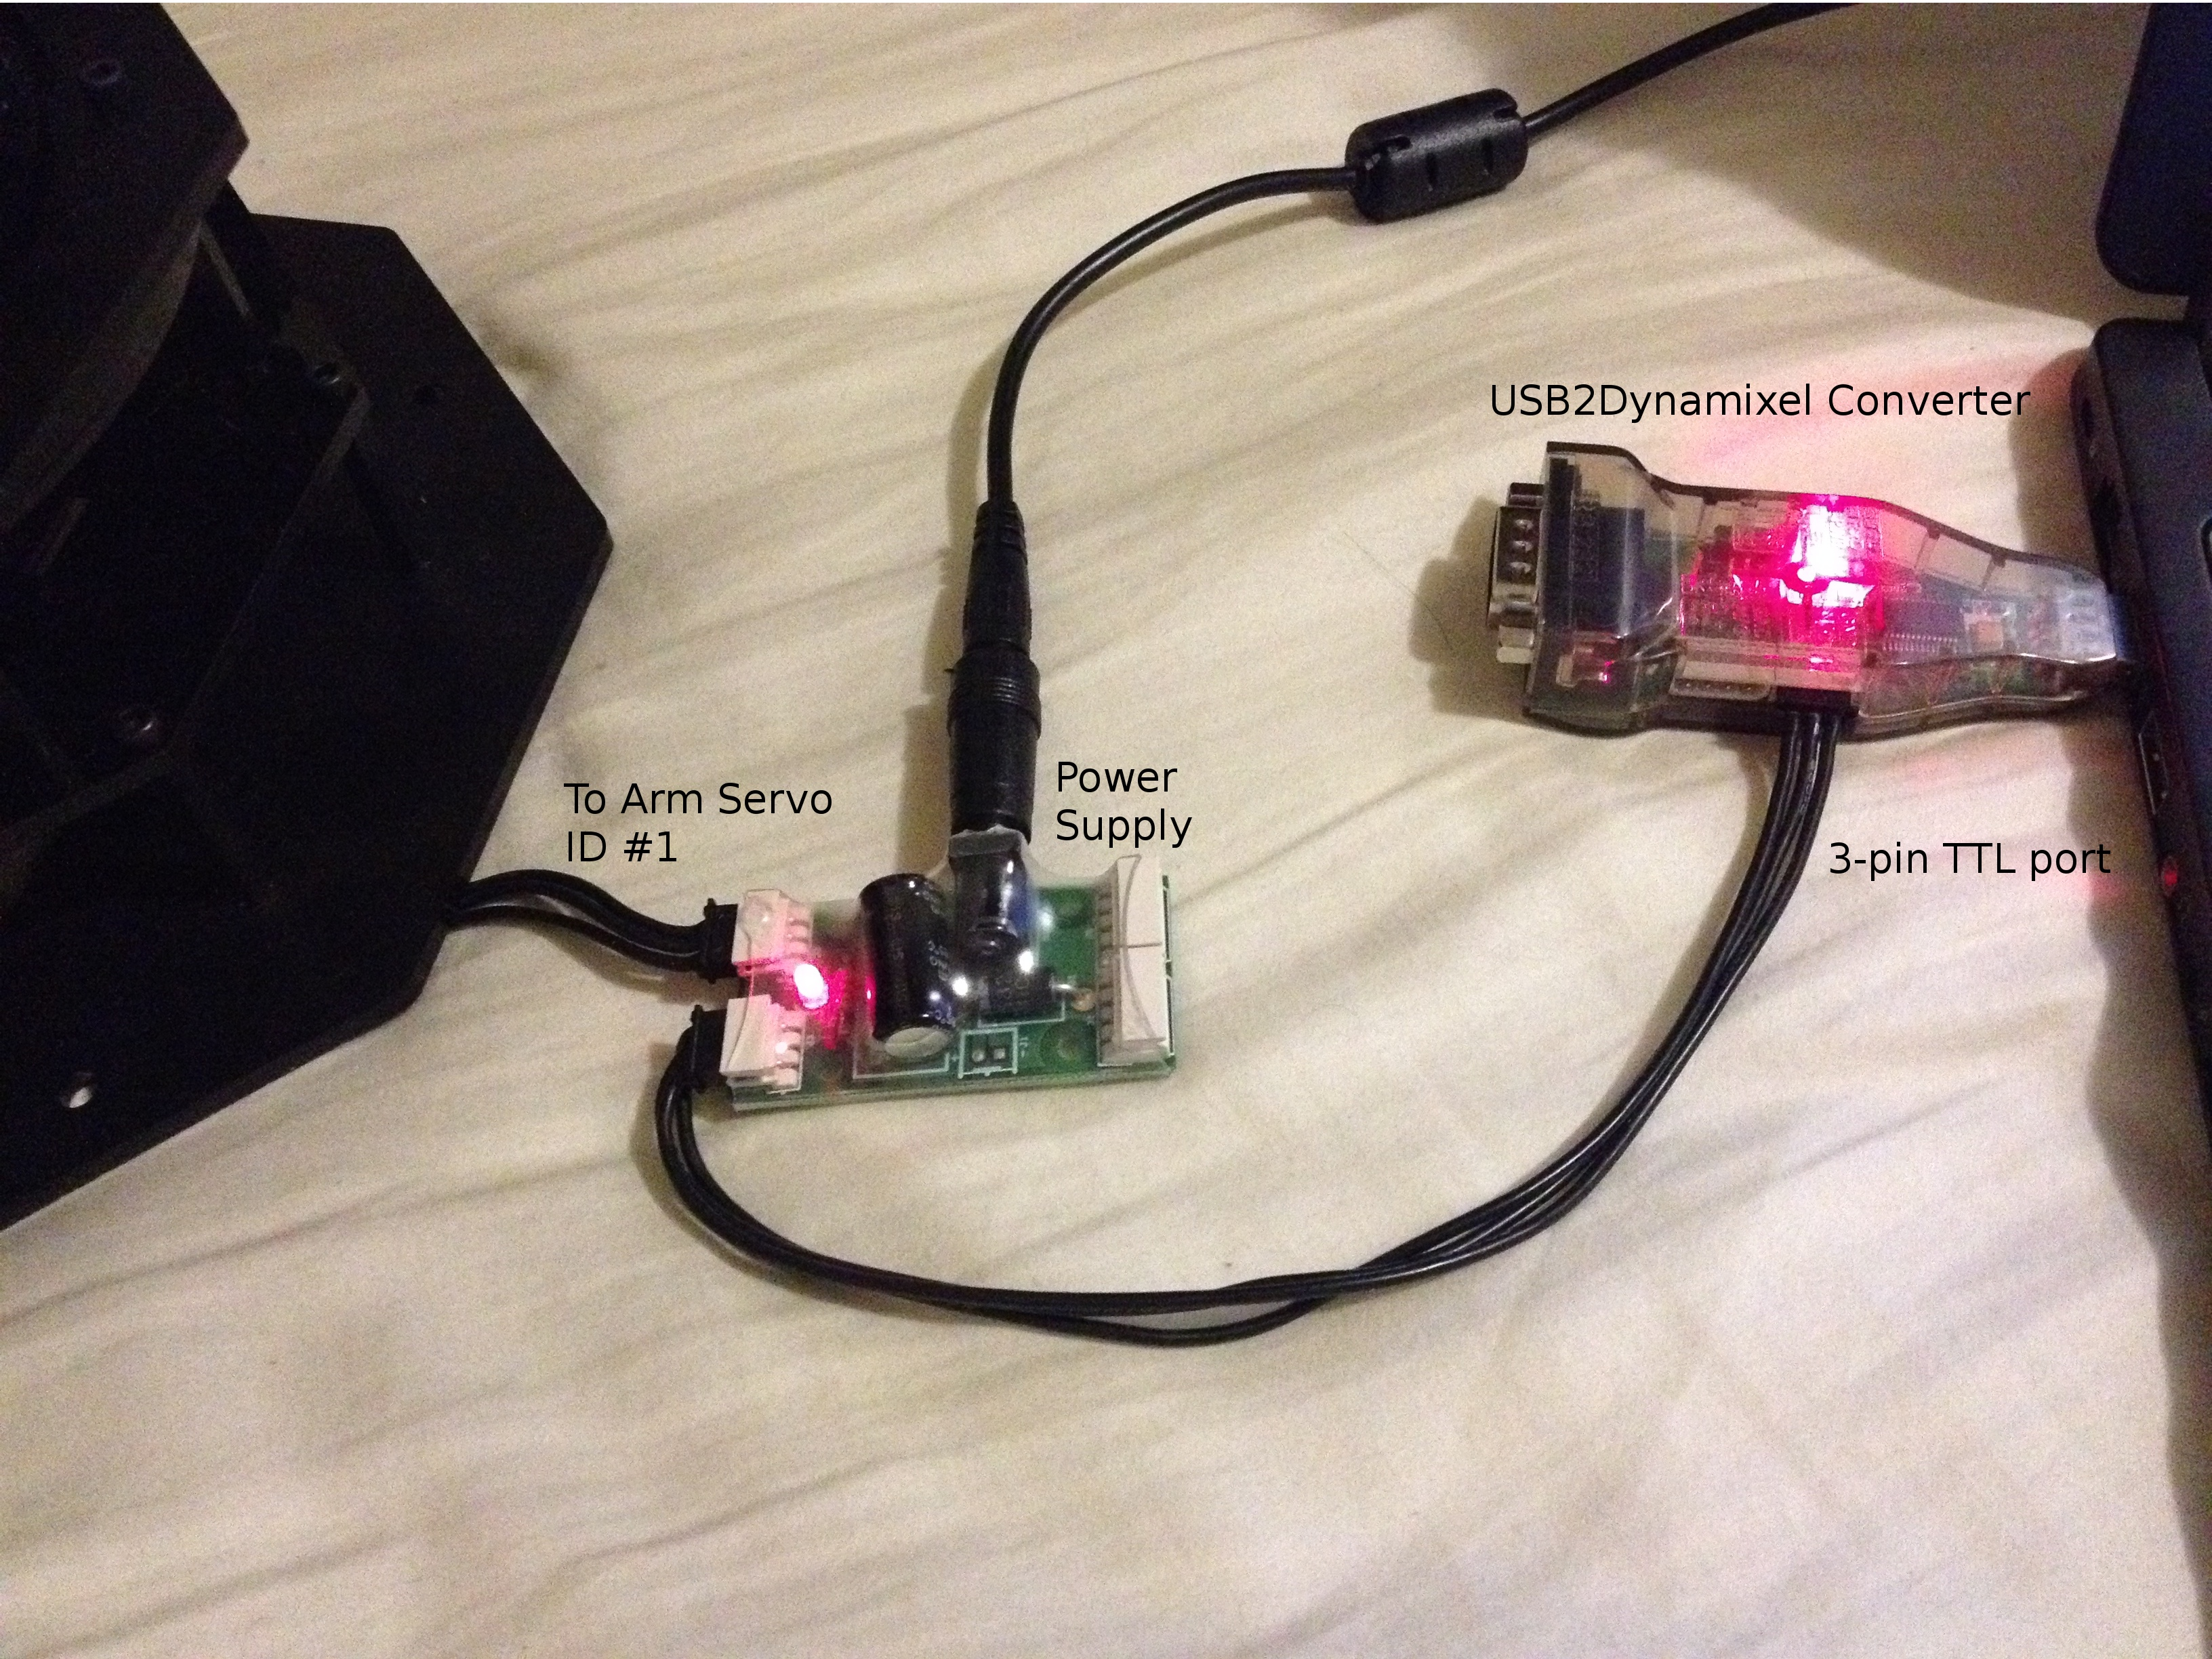
\includegraphics[width=10.0cm]{resources/usb2dxl-connections-labeled}
	\end{center}
    \begin{itemize}
      \item Plugged USB2Dynamixel adapter into the USB-3 port on my computer
      \item Connected the TTL 3-pin port on the adapter to one of the 3-pin ports on the SMPS2Dynamixel power adapter
      \item Connected the other 3-pin port on the SMPS2Dynamixel power adapter to the Dynamixel motor with ID 1
      \item Plugged the Reactor arm AC adapter into the SMPS2Dynamixel power adapter using the 2.1mm-to-2.5mm DC power plug adapter
    \end{itemize}
  \subsection{Identifying the Motors with ROS}
    \begin{itemize}
      \item Following the ROS dynamixel\_controllers tutorial "Connecting to Dynamixel Bus" I created a new ros package with "roscreate-pkg  my\_dynamixel\_tutorial dynamixel\_controllers" and created a launch file in the package that pings the motor IDs specified and displays the motors that it found (\url{http://wiki.ros.org/dynamixel_controllers/Tutorials/
ConnectingToDynamixelBus})
      \item The output was \newline
      [INFO] [WallTime: 1400874215.506928] arm\_port: Pinging motor IDs 1 through 8... \newline
      [INFO] [WallTime: 1400874215.949469] arm\_port: Found 8 motors - 8 AX-12 [1, 2, 3, 4, 5, 6, 7, 8], initialization complete.
      \item rostopic echo /motor\_state/arm\_port displayed all the state feedback for the motors
    \end{itemize}
  \subsection{Creating a Joint Position Controller}
    \begin{itemize}
      \item Following the ROS dynamixel\_controllers tutorial "Creating a joint controller" I created a joint controller for the base servo (ID \#1). This allows you to set the type of controller, joint speed, and motor ID, min, max and init angle values. (\url{http://wiki.ros.org/dynamixel\_controllers/Tutorials/CreatingJointPositionController})
      \item The output was \newline
      process[base\_controller\_spawner-1]: started with pid [25011] \newline
[INFO] [WallTime: 1405234746.116965] arm\_port controller\_spawner: waiting for controller\_manager dxl\_manager to startup in global namespace... \newline
[INFO] [WallTime: 1405234746.126165] arm\_port controller\_spawner: All services are up, spawning controllers... \newline
[INFO] [WallTime: 1405234746.202863] Controller base\_controller successfully started. \newline
[base\_controller\_spawner-1] process has finished cleanl
    \end{itemize}
% -------------------------------------------------------------------------------------
% REFERENCES
% -------------------------------------------------------------------------------------
%\bibliography{}

% -------------------------------------------------------------------------------------
% END DOCUMENT
% -------------------------------------------------------------------------------------
\end{document}
